\documentclass[spanish]{beamer}
\usepackage[utf8]{inputenc}
\usepackage[spanish]{babel}
\usefonttheme{professionalfonts}% font de LaTeX
%~ \usetheme{UNLTheme}
%~ \usepackage[latin1]{inputenc}
\usepackage{latexsym} % Símbolos
\usepackage{amsmath}
\usepackage{amssymb}
\usepackage{eurosym}
\usepackage{eso-pic}
\usepackage{graphicx}
\usetheme{Hannover}
\usecolortheme{whale}
%~ \setbeamercolor{itemize item}{fg=darkred!80!black}

\begin{document}
\title{OMI}
% Sin pagina de titulo
%~ \frame{\titlepage}

%%Fondo título:
\usebackgroundtemplate{\AddToShipoutPicture{\put(\LenToUnit{.3\paperwidth},\LenToUnit{.4\paperheight}){
\includegraphics[scale=2]{img/logo-doc.png}}}}
\begin{frame}
\hfill \\
\hfill \\
\hfill \\
\hfill \\
\hfill \\
\hfill \\
\hfill \\
\hfill \\
\hfill \\
\hfill \\
\hfill \\
\hfill \\
\hfill \\
\hfill \\
\begin{itemize}
        \item \textbf{Fco. Javier Bohórquez Ogalla}
        \item \textbf{Ingeniería técnica en informática de sistemas}
        \item \textbf{Escuela superior de Ingeniería (UCA)}
    \end{itemize}
\end{frame}

%%Fondo trikker
%\usebackgroundtemplate{\AddToShipoutPicture{\put(\LenToUnit{.12\paperwidth},\LenToUnit{.0\paperheight}){\includegraphics[scale=0.40]{img/tri.jpg}}}}
%\begin{frame}{}
%\end{frame}

%%Fondo Urgol
%\usebackgroundtemplate{\AddToShipoutPicture{\put(\LenToUnit{.12\paperwidth},\LenToUnit{.0\paperheight}){\includegraphics[scale=0.40]{img/urg.jpg}}}}
%\begin{frame}{}
%\end{frame}

%Fondo Lunari
%\usebackgroundtemplate{\AddToShipoutPicture{\put(\LenToUnit{.12\paperwidth},\LenToUnit{.0\paperheight}){\includegraphics[scale=0.40]{img/lun.jpg}}}}
%\begin{frame}
%\end{frame}

%Fondo Blanco
%\usebackgroundtemplate{\AddToShipoutPicture{\put(\LenToUnit{.12\paperwidth},\LenToUnit{.0\paperheight}){
\includegraphics[scale=3]{img/background.jpg}}}}
%\begin{frame}
%\end{frame}

%%%%%%%%%%%%%%%%%%%%%%%%%%%%%%%%%%%%%%%%%%%%%%%%%%%%%%%%%%%%%%%%%%%%%%%%%%%%%%%%%%%%%%%%%%%%%%%%%%%%%%%%%%
%% Diapositivas                                                                                         %%
%%%%%%%%%%%%%%%%%%%%%%%%%%%%%%%%%%%%%%%%%%%%%%%%%%%%%%%%%%%%%%%%%%%%%%%%%%%%%%%%%%%%%%%%%%%%%%%%%%%%%%%%%%

\section{Introducción}
\usebackgroundtemplate{\AddToShipoutPicture{\put(\LenToUnit{.12\paperwidth},\LenToUnit{.0\paperheight}){
\includegraphics[scale=3]{img/background.jpg}}}}
\begin{frame}{Introducción}
    \begin{itemize}
        \item Conjunto de herramientas.
        \item Ayudan en el aprendizaje:
        \begin{itemize}
            \item Teoría de intérpretes.
            \item Lenguajes formales.
        \end{itemize}
         \item Facilita el estudio por medio de:
         \begin{itemize}
            \item Interactividad.
            \item Documentación.
        \end{itemize}
    \end{itemize}
\end{frame}


\begin{frame}{Motivación}
    \begin{itemize}
        \item Limitaciones en cursos académicos.
        \item No existe: 
        \begin {itemize}
            \item Caso práctico $\Rightarrow$ aplicación completa de los conceptos estudiados.
            \item Herramienta interactiva $\Rightarrow$ funcionamiento de los sistemas intérpretes.
        \end{itemize}
   \end{itemize}
\end{frame}

\begin{frame}{Alcance: Intérprete OMI}
    \begin{itemize}
        \item Sistema software capaz de analizar y ejecutar otros programas escritos en un lenguaje específico.
        \item Procesa código fuente desde: 
        \begin {itemize}
            \item Entrada estándar
            \item Fichero
            \item Una consola interactiva (prompt)
            \item Puerto TCP  
        \end{itemize}
        \item Varios modos de ejecución: 
        \begin {itemize}
            \item Consola interactiva
            \item Servidor
            \item Salida de datos que detalla el proceso
        \end{itemize}
         \item Extendido, configurado y personalizado por medio de:
         \begin {itemize}
            \item Módulos
            \item Opciones de compilación
        \end{itemize}
   \end{itemize}
\end{frame}

\begin{frame}{Alcance: Lenguaje OMI}
    \begin{itemize}
      \item Multiparadigma 
      \item Alto nivel
      \item Propósito general
      \item Tipado dinámico
      \item Sintaxis sencilla y cercana a los lenguajes actuales
      \item Tipos de datos simples y compuestos
      \item Operadores sobre los tipos de datos
      \item Variables locales y globales
      \item Estructuras y sentencias de control de flujo
      \item Características de la programación funcional
      \item Características de la programación orientadas a objetos
      \item Reflexión
      \item Introspección de tipos
      \item Funciones para la manipulación de:
      \begin{itemize}
         \item Ficheros
          \item Procesos
          \item Fechas
      \end{itemize}
   \end{itemize}
\end{frame}

\begin{frame}{Alcance: Módulo OMI}
    \begin{itemize}
      \item Desarrollo de un módulo y documentación del proceso.
      \item Módulo para la internacionalización y localización: gettext
   \end{itemize}
\end{frame}

\begin{frame}{Alcance: Biblioteca de desarrollo OMI}
    \begin{itemize}
      \item Recursos de programación sobre el que se construye el intérprete
      \item Puede ser instalada de forma independiente
      \item Puede ser utilizada para construir:
      \begin{itemize}
         \item Módulos OMI
         \item Software que necesite interpretar código OMI
      \end{itemize}
   \end{itemize}
\end{frame}
%~ 

\begin{frame}{Alcance: Sitio web del proyecto OMI}
    \begin{itemize}
      \item omi-project.com
      \item Presentación del proyecto
      \item Medio de acceso a la documentación y el software desarrollado
   \end{itemize}
\end{frame}

\begin{frame}{Alcance: runTree}
    \begin{itemize}
      \item Herramienta online. Permite escribir e interpretar código OMI
      \item Describe el árbol sintáctico y el proceso de ejecución paso a paso del mismo
      \item Detalla el estado interno y la entrada/salida de datos
      \item Cliente del intérprete OMI
   \end{itemize}
\end{frame}

\section{Estado del arte}
\begin{frame}{Estado del arte}
    \begin{itemize}
      \item Conceptos y estudios previos.
      \item Comparativa de herramientas 
      \begin{itemize}
      \item Funcionalidades
      \item Características
      \end{itemize}
   \end{itemize}
\end{frame}

\section{Planificación}
\begin{frame}{Metodología}
    \begin{itemize}
      \item Iterativa e incremental
      \item Proceso unificado de desarrollo de software 
      \begin {itemize}
         \item Dirigido por casos de uso 
         \item Centrado en la arquitectura
      \end{itemize}
      \item Enfoque en espiral, dividido en cuatro etapas:
      \begin {itemize}
         \item Deterrminar objetivos
         \item Análisis de riesgos
         \item Desarrollo
         \item Planificación
      \end{itemize}
      \item UML
   \end{itemize}
\end{frame}

\begin{frame}{Planificación}
    \begin{itemize}
      \item Se divide en iteraciones
      \item Cada iteración:
      \begin {itemize}
         \item Objetivos
         \item Riesgos
         \item Desarrollo
         \begin{itemize}
         \item Análisis
         \item Diseño
         \item Codificación
         \item Pruebas
         \end{itemize}
         \item Planificación
      \end{itemize}
      \item Punto de partida: 03/11/2014
      \item Jornada laboral de 8 horas y 5 días hábiles
      \item Diagrama de Gantt general
   \end{itemize}
\end{frame}

\begin{frame}{Organización y costes}
    \begin{itemize}
      \item Único empleado  
      \begin{itemize}
         \item Salario anual bruto de 18120\euro (BOE 30 de noviembre de 2013)
         \item 8 meses de trabajo  12.080,00\euro
      \end{itemize}
      \item Único equipo
      \begin{itemize}
         \item Prestaciones medias
         \item 409\euro
      \end{itemize}
   \end{itemize}
\end{frame}

\begin{frame}{Organización y costes}
   \tiny {
    \begin{description}
      \item [Sistema operativo:] GNU/Linux. 
      \item [Entorno integrado de desarrollo:] Geany.
      \item [Generador léxico:] Flex.
      \item [Generador sintáctico:] Bison.
      \item [Compilador:] GCC.
      \item [Depurador:] GDB.
      \item [Herramientas para la construcción automática:] Autoconf, automake, make.
      \item [Desarrollo de diagramas:] Dia, railroad diagram generator.
      \item [Control de versiones:] Subversion.
      \item [Creación de documentación:] Latex, Doxygen.
      \item [Planificación:] Planner.
      \item [Bibliotecas de desarrollo:] readline, boost. 
      \item [Servidor HTTP: ] Apache.
      \item [Intérprete de Scripts de servidor:] PHP.
      \item [Navegador web:] Firefox, Chrome, Explorer.
      \item [Conversor latex a HTML:] latex2html.
      \item [Editor gráfico:] Gimp, Inkscape.
      \item [Comunicación:] Servicio gratuito de correo electrónico. 
      \end{description}
      }
\end{frame}

\begin{frame}{Riesgos}
    \begin{itemize}
      \item Identifica los riesgos  
      \begin{itemize}
         \item Probabilidad
         \item Impacto
      \end{itemize}
      \item Define planes seguidos
      \begin{itemize}
         \item Reducir efectos
         \item Disminuir la probabilidad 
      \end{itemize}
      \item Según su tipo
      \begin{itemize}
         \item Riesgos tecnológicos
         \item Riesgos de requisitos
         \item Riesgos de soluciones
         \item Riesgos de costes, tiempos y recurso
      \end{itemize}
   \end{itemize}
\end{frame}

\begin{frame}{Calidad}
    \begin{itemize}
      \item Norma ISO 9000
      \item Formado procesos
      \begin{itemize}
         \item Ingresan requisitos
         \item Obtiene un producto que cumple los requisitos y satisface el cliente
      \end{itemize}
   \end{itemize}
\end{frame}

\section{Requisitos del sistema}
\begin{frame}{Situación actual}
    \begin{itemize}
      \item Análisis del proceso de aprendizaje en la teoría de autómatas, lenguajes formales e intérpretes. 
      \item Centrado en cursos académicos
      \item Conclusión:
      \begin{itemize}
         \item Limitaciones de tiempo
         \item No disponen de un caso práctico completo
         \item No disponen de herramientas interactivas
      \end{itemize}
   \end{itemize}
\end{frame}

\begin{frame}{Necesidades}
    \begin{itemize}
      \item Herramientas interactivas que ayuden a ver cómo funciona y se construye un intérprete. 
      \item Documentación detallada y accesible 
   \end{itemize}
\end{frame}

\begin{frame}{Objetivos}
    \begin{itemize}
      \item Intérprete para un lenguaje de programación
      \begin{itemize}
         \item Características actuales y avanzadas
         \item Interactivo
         \item Detalla el proceso de interpretación
      \end{itemize}
      \item Documentación detallada, estructurada y accesible
      \item Aplicación web que aloje todos los recursos del proyecto
      \item Biblioteca de desarrollo
      \item Herramienta online que haga uso del intérprete y muestre gráficamente el proceso
   \end{itemize}
\end{frame}

\begin{frame}{Requisitos funcionales}
    \begin{itemize}
      \item Centrados en:
      \begin{itemize}
         \item Intérprete
         \item Lenguaje OMI
         \item Web
         \item Biblioteca de desarrollo OMI
         \item Cliente OMI (runTree)
      \end{itemize}
      \item 189 requisitos funcionales.
   \end{itemize}
\end{frame}

\begin{frame}{Requisitos no funcionales}
    \begin{itemize}
      \item Rendimiento 
      \begin{itemize}
      \item Tiempo
      \item Espacio
      \end {itemize}
      \item Usabilidad
      \item Accesibilidad
      \item Estabilidad
      \item Mantenibilidad
      \item Concurrencia
   \end{itemize}
\end{frame}

\section{Análisis del sistema}
\begin{frame}{Modelo conceptual}
    \begin{itemize}
      \item Organizado en paquetes
      \begin{itemize}
      \item General
      \item Intérprete
      \item Nodo ejecutable
      \item Tipos de datos
      \item Error
      \item Extensiones
      \item Tipos de nodos ejecutables
      \item runTree
      \end {itemize}
   \end{itemize}
\end{frame}

\begin{frame}{Modelo de casos de uso: Intérprete}
    \begin{center}
      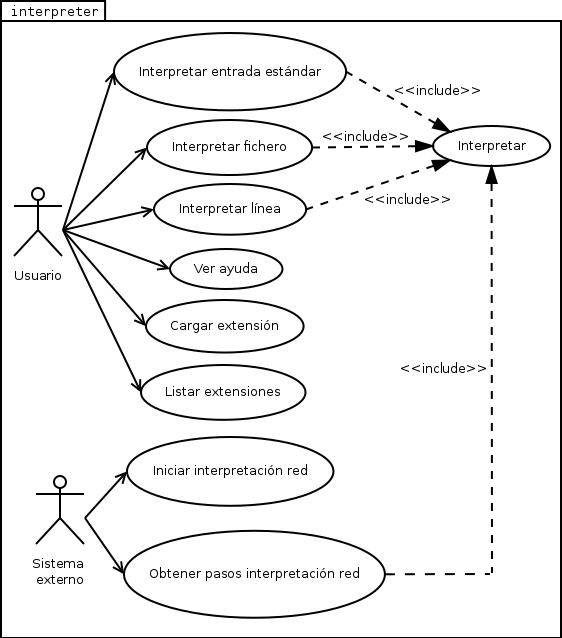
\includegraphics[scale=0.3]{use_case_interpreter.png} 
      \end{center}
\end{frame}


\begin{frame}{Modelo de casos de uso: runTree}
   \begin{center}
      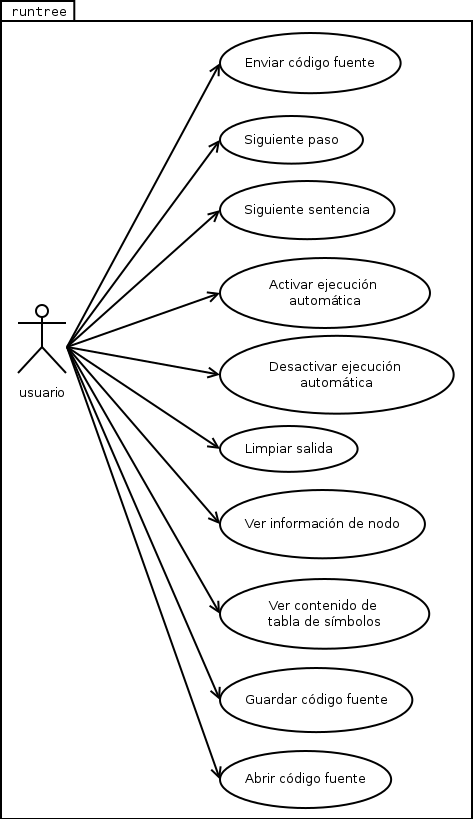
\includegraphics[scale=0.25]{runtree.png}
   \end{center}
\end{frame}

\begin{frame}{Modelo comportamiento del sistema: Diagramas de secuencia}
   \begin{itemize}
      \item Casos de usos $\Rightarrow$ diagramas de secuencia $\Rightarrow$ eventos y valores retorno
      \item Interprete
      \begin{itemize}
         \item Iniciar el interprete
         \item Recibir código fuente diferentes medios
         \item No relacionados interpretación
      \end{itemize}
      \item runTree
      \begin{itemize}
         \item Enviar código fuente para interpretación
         \item Obtener pasos en la interpretación 
         \item Interfaz y navegación
      \end{itemize}
   \end{itemize}
\end{frame}

\begin{frame}{Modelo comportamiento del sistema: Contrato de operaciones}
   \begin{itemize}
      \item Interprete
      \begin{itemize}
         \item Analizador léxico
         \item Analizador sintáctico
         \item Tablas de símbolos
         \item Nodos ejecutables
      \end{itemize}
      \item runTree
      \begin{itemize}
         \item Crea entidades similares al intérprete
         \item Refleja el estado interno del intérprete
      \end{itemize}
   \end{itemize}
\end{frame}

\begin{frame}{Modelo de interfaz de usuario}
   \begin{itemize}
      \item Interprete
      \begin{itemize}
         \item Consola de comandos
         \item Entrada del teclado en forma de comandos y opciones 
         \item Salida en formato textual
      \end{itemize}
      \item runTree
      \begin{itemize}
         \item Accesible desde navegador web
         \item Elementos:
         \begin {itemize}
            \item Código fuente
            \item Árbol sintáctico
            \item Tablas de símbolos
            \item I/O del programa
            \item Consola informativa
         \end {itemize}
      \end{itemize}
      \item Web
      \begin{itemize}
         \item Diagrama de navegación
      \end{itemize}
   \end{itemize}
\end{frame}

\section{Diseño del Sistema}
\begin{frame}{Arquitectura física}
   \begin{itemize}
      \item Escritorio 
      \begin{itemize}
         \item Comando del S.O.
      \end{itemize}
      \item Cliente/Servidor
      \begin{itemize}
         \item Intérprete hace de servidor
         \item Otros sistemas hacen de cliente (runTree)
         \item Código fuente desde puerto TCP
         \item Cada petición produce JSON que describe un paso.
      \end{itemize}
   \end{itemize}
\end{frame}
\begin{frame}{Arquitectura lógica: Intérprete}
   \begin{itemize}
         \item Front-end
         \begin{itemize}
             \item Componentes I/O
             \item Analizador léxico 
             \item Analizador sintáctico
         \end{itemize}
         \item Back-end
         \begin{itemize}
            \item Nodos ejecutables
            \item Tabla de símbolos
         \end{itemize}
      \end{itemize}
\end{frame}
\begin{frame}{Arquitectura lógica: runTree}
   \begin{itemize}
         \item Front-end
         \begin{itemize}
             \item Componentes I/O
         \end{itemize}
         \item Back-end
         \begin{itemize}
            \item Comunicación con el servidor
         \end{itemize}
      \end{itemize}
\end{frame}

\begin{frame}{Gramática}
   \begin{itemize}
         \item Libre de contexto
         \item Se describe:
         \begin{itemize}
            \item Diagramas de carril
            \item Lenguaje EBNF
         \end{itemize}
   \end{itemize}
\end{frame}

\begin{frame}{Comunicaciones}
   \begin{itemize}
         \item Estructura JSON que devuelve el servidor 
         \item Se describe:
         \begin{itemize}
            \item Esquemas JSON (json-schema.org)
         \end{itemize}
   \end{itemize}
\end{frame}

\begin{frame}{Componentes}
   \begin{itemize}
         \item Interacción y comunicación entre objetos.
         \item Diagrama de secuencia: interpretar código fuente
         \item Diagramas de comunicación: sentencias OMI 
   \end{itemize}
\end{frame}

\begin{frame}{Interfaz de usuario}
   \begin{itemize}
         \item Comando OMI
         \begin {itemize}
            \item Opciones y argumentos
            \item Modos de ejecución
         \end{itemize}
         \item runTree
         \item Web del proyecto 
   \end{itemize}
\end{frame}

\section{Construcción del sistema}
\begin{frame}{Construcción del sistema}
   \begin{itemize}
         \item Herramientas software utilizadas
         \item Ficheros de código fuente
         \item Fragmentos de código fuente
   \end{itemize}
\end{frame}

\section{Pruebas del sistema}
\begin{frame}{Pruebas del sistema}
   \begin{itemize}
         \item Estrategia: en cada iteración pruebas de caja negra 
         \item Entorno de pruebas
         \item Roles: único usuario
         \item Niveles de pruebas
         \begin{itemize}
            \item Pruebas unitarias
            \item Pruebas de integración
            \item Pruebas funcionales
            \item Pruebas no funcionales
         \end{itemize}
   \end{itemize}
\end{frame}

\section{Manual de implantación}
\begin{frame}{Manual de implantación}
   \begin{itemize}
         \item Configuración del entorno hardware y software
         \begin {itemize}
            \item Servidor de nombre de dominios
            \item Servido web
            \item Intérprete OMI
            \item Web del proyecto
         \end{itemize}
         \item Pruebas de implantación
   \end{itemize}
\end{frame}

\section{Manual de usuario}
\begin{frame}{Manual de usuario}
   \begin{itemize}
         \item Características
         \item Requisitos previos
         \item Uso de los sistemas
         \begin {itemize}
            \item Obtener el software
            \item Instalación
            \item Intérprete  OMI
            \item Referencias del lenguaje OMI
            \item Extensiones del lenguaje
            \item Funcionamiento cliente/servidor
            \item Modo de ejecución detallado
            \item runTree
         \end{itemize}
   \end{itemize}
\end{frame}

\section{Conclusiones}
\begin{frame}{Conclusiones}
   \begin{itemize}
         \item Objetivos
         \item Lecciones aprendidas
         \item Trabajo futuro
   \end{itemize}
\end{frame}

\section{Bibliografía}
\begin{frame}{Bibliografía}
   \tiny{
   Referencias bibliográficas:
\begin{itemize}
\item Compiladores y procesadores del lenguaje (José Antonio Jiménez Millám) [Servicios publicaciones universidad de Cádiz].
\item Compiladores. Principios, técnicas y herramientas 2ªed. (Alfred Aho, Ravi Sethi, Jeffrey Ullman y Monica S. Lam) [Pearson Addison Wesley].
\item El lenguaje unificado de modelado (Booch, Rumbaugh y Jacobson) [Pearson Addison Wesley].
\end{itemize}

Portales webs sobre lenguajes de programación:
\begin{itemize}
\item isocpp.org: Estándar C++.
\item cplusplus.com: C++ referencias y tutoriales.
\item docs.oracle.com: Java Platform, Standard Edition.
\item php.net: PHP documentación y referencias.
\item python.org: Python documentación y referencias.
\item ruby-lang.org: Ruby documentación y referencias.
\item w3schools.com: JavaScript tutoriales y referencias W3C.
\item developer.mozilla.org: JavaScript tutoriales y referencias Mozilla.
\item nodejs.org: Node.js documentación y referencias.
\item uam.es: Manual básico LISP.
\item haskell.org: Haskell documentación y referencias.
\item swi-prolog.org: Prolog documentación y referencias.
\item perl.org: Perl documentación y referencias.
\item scala-lang.org: Scala documentación y referencias.
\end{itemize}
\pagebreak
Otros recursos generales:
\begin{itemize}
\item wikipedia.org
\item stackoverflow.com
\end{itemize}
   }
\end{frame}

\section{Licencia}
\begin{frame}{Licencia}
   \begin{itemize}
         \item Software: GPLv3.
         \item Documentación: Creative Commons.
   \end{itemize}
\end{frame}


%~ 
%~ \section{Diseño Gráfico}
%~ \usebackgroundtemplate{\AddToShipoutPicture{\put(\LenToUnit{.12\paperwidth},\LenToUnit{.0\paperheight}){
\includegraphics[scale=3]{img/background.jpg}}}}
%~ \begin{frame} {Primeros bocetos}
    %~ \begin{center}
        %~ \includegraphics[scale=0.37]{img/bocetos.png}\\
        %~ Bocetos de distintas criaturas\\
    %~ \end{center}
%~ \end{frame}
%~ 
%~ \usebackgroundtemplate{\AddToShipoutPicture{\put(\LenToUnit{.12\paperwidth},\LenToUnit{.0\paperheight}){
\includegraphics[scale=3]{img/background.jpg}}}}
%~ \begin{frame} {Resultados finales}
    %~ \begin{center}
        %~ \includegraphics[scale=0.3]{img/erlic.png}\\
        %~ Rejilla final Erlic\\
        %~ \includegraphics[scale=0.3]{img/object_istelgar.png}\\
        %~ Rejilla objetos
    %~ \end{center}
%~ \end{frame}
%~ 
%~ \section {R-GeL}
%~ \usebackgroundtemplate{\AddToShipoutPicture{\put(\LenToUnit{.12\paperwidth},\LenToUnit{.0\paperheight}){
\includegraphics[scale=3]{img/background.jpg}}}}
%~ \begin{frame} {Motor Gráfico}
    %~ \begin{center}
        %~ \includegraphics[scale=0.30]{img/r_gel_logo.png}\\
        %~ Retro Game Engine Library
    %~ \end{center}    
%~ \end{frame}
%~ 
%~ \usebackgroundtemplate{\AddToShipoutPicture{\put(\LenToUnit{.12\paperwidth},\LenToUnit{.0\paperheight}){
\includegraphics[scale=3]{img/background.jpg}}}}
%~ \begin{frame} {Diagrama}
    %~ \begin{center}
        %~ \includegraphics[scale=0.25]{img/r_gel_dia.jpeg}\\
        %~ \begin{itemize}
            %~ \item Sistema de capas 
            %~ \item Control de colisiones
            %~ \item Funciones
        %~ \end{itemize}        
    %~ \end{center}    
%~ \end{frame}
%~ 
%~ \section {I.A.}
%~ \usebackgroundtemplate{\AddToShipoutPicture{\put(\LenToUnit{.12\paperwidth},\LenToUnit{.0\paperheight}){\includegraphics[scale=0.40]{img/urg.jpg}}}}
%~ \begin{frame} {Modelo de I.A.}
    %~ \begin{center}
        %~ \includegraphics[scale=0.25]{img/ia_dia.jpeg}\\
        %~ \begin{itemize}
            %~ \item Estados del juego
            %~ \item Busca estado ganador
            %~ \item Valoración del entorno
        %~ \end{itemize}        
        %~ 
    %~ \end{center}    
%~ \end{frame}
%~ 
%~ \section{Problemas}
%~ \usebackgroundtemplate{\AddToShipoutPicture{\put(\LenToUnit{.12\paperwidth},\LenToUnit{.0\paperheight}){
\includegraphics[scale=3]{img/background.jpg}}}}
%~ \begin{frame} {Problemas encontrados...}
    %~ \begin{itemize}
            %~ \item \textbf{Motor gráfico}
                %~ \begin{itemize}
                    %~ \item[] \underline{\textit{Problema:}} A la hora de pintar un objeto...puede afecta a los demás.
                    %~ \item[] \underline{\textit{Solución:}} Crear nuestro motor gráfico \textbf{propio}.
                %~ \end{itemize}
            %~ \item \textbf{Sistema de colisiones}
                %~ \begin{itemize}
                    %~ \item[] \underline{\textit{Problema:}} Las colisiones por posicionamiento en tiles...es una mala idea, hay falta de realismo.
                    %~ \item[] \underline{\textit{Solución:}} Definir \textbf{áreas de colisión} para cada elemento.
                %~ \end{itemize}
            %~ \item \textbf{Decorados}
                %~ \begin{itemize}
                    %~ \item[] \underline{\textit{Problema:}} Que los objetos forman parte del mapa...es un quebradero de cabeza a la hora de estudiar las colisiones.
                    %~ \item[] \underline{\textit{Solución:}} \textbf{Distintas} rejillas para el terreno y los objetos del mapa.
                %~ \end{itemize}
    %~ \end{itemize} 
%~ \end{frame}
%~ 
%~ \section {Beta}
%~ \usebackgroundtemplate{\AddToShipoutPicture{\put(\LenToUnit{.12\paperwidth},\LenToUnit{.0\paperheight}){\includegraphics[scale=0.40]{img/tri.jpg}}}}
%~ \begin{frame}{Beta}
    %~ \begin{center}
        %~ Y ahora, lo importante, \textbf{¡¡Una beta jugable!!}
    %~ \end{center}
%~ \end{frame}

\end{document}
